%!TEX root = ../presentation.tex


% -------------- BACKGROUNDS --------------

\newcommand\titlebackground {
    \usebackgroundtemplate{
    \begin{tikzpicture}[remember picture, overlay]
        \node[at=(current page.center)] {
            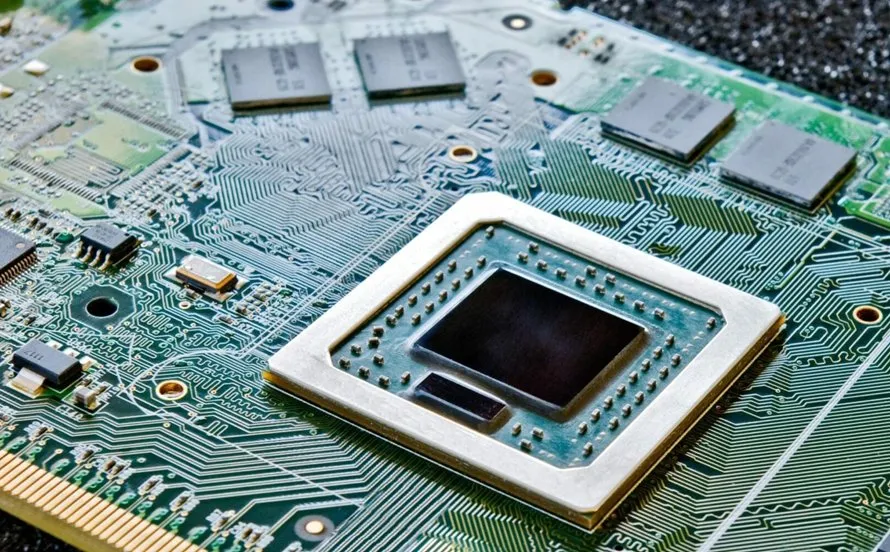
\includegraphics
            [width=\paperwidth, keepaspectratio]
            {pictures/background/background-PCB.png}
        };
    \end{tikzpicture}
    }
}


\newcommand\introbackground {
    \usebackgroundtemplate{
    \begin{tikzpicture}[remember picture, overlay]
        \node[at=(current page.center)] {
            
\includegraphics
            [width=\paperwidth, keepaspectratio]
            {pictures/background/background-pcb-poster.png}
        };
    \end{tikzpicture}
    }
}

\newcommand\pausebackground {
    \usebackgroundtemplate{
    \begin{tikzpicture}[remember picture, overlay]
        \node[at=(current page.center)] {
            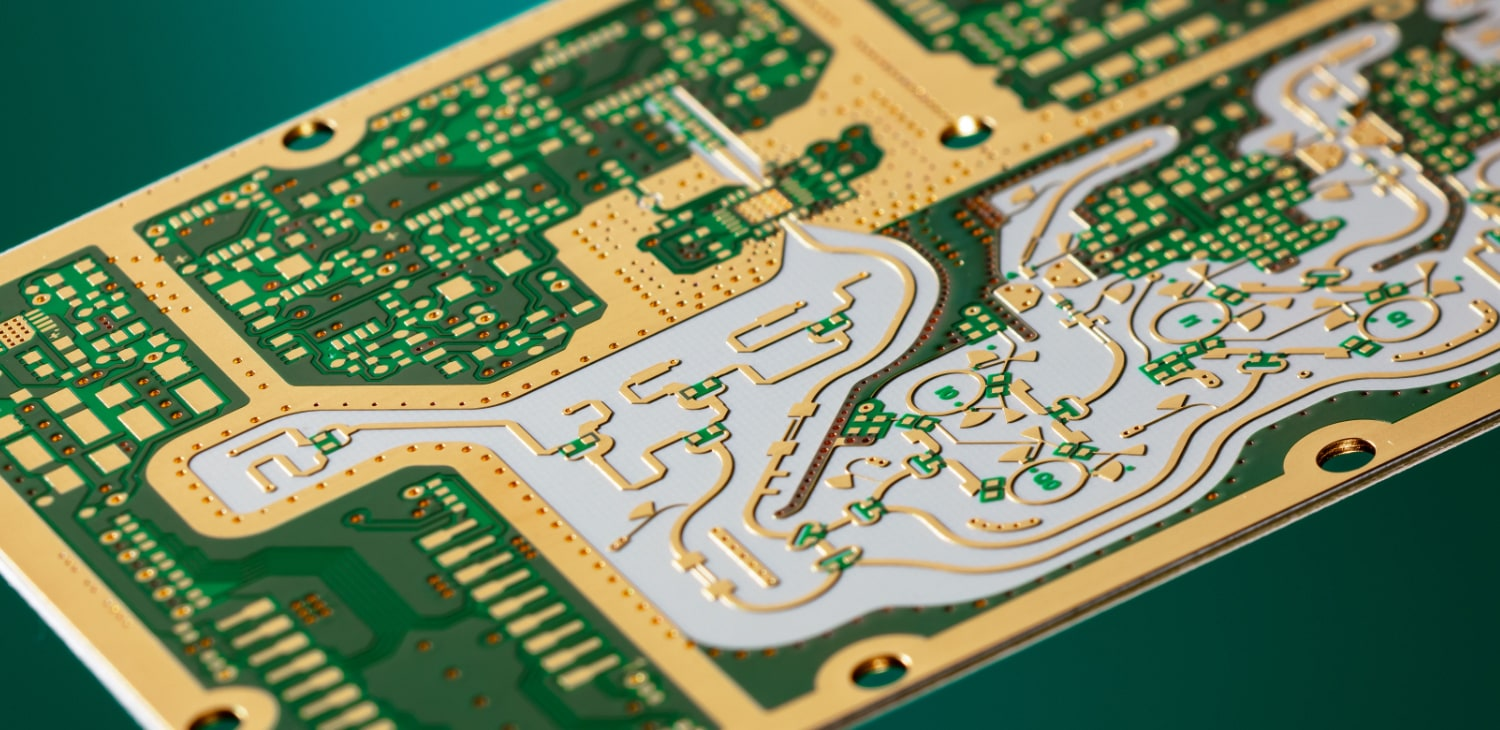
\includegraphics
            [height=\paperheight, keepaspectratio]
            {pictures/background/background-level-A.jpg}
        };
    \end{tikzpicture}
    }
}

\newcommand\chapterbackground {
    \usebackgroundtemplate{
    \begin{tikzpicture}[remember picture, overlay]
        \node[at=(current page.center)] {
            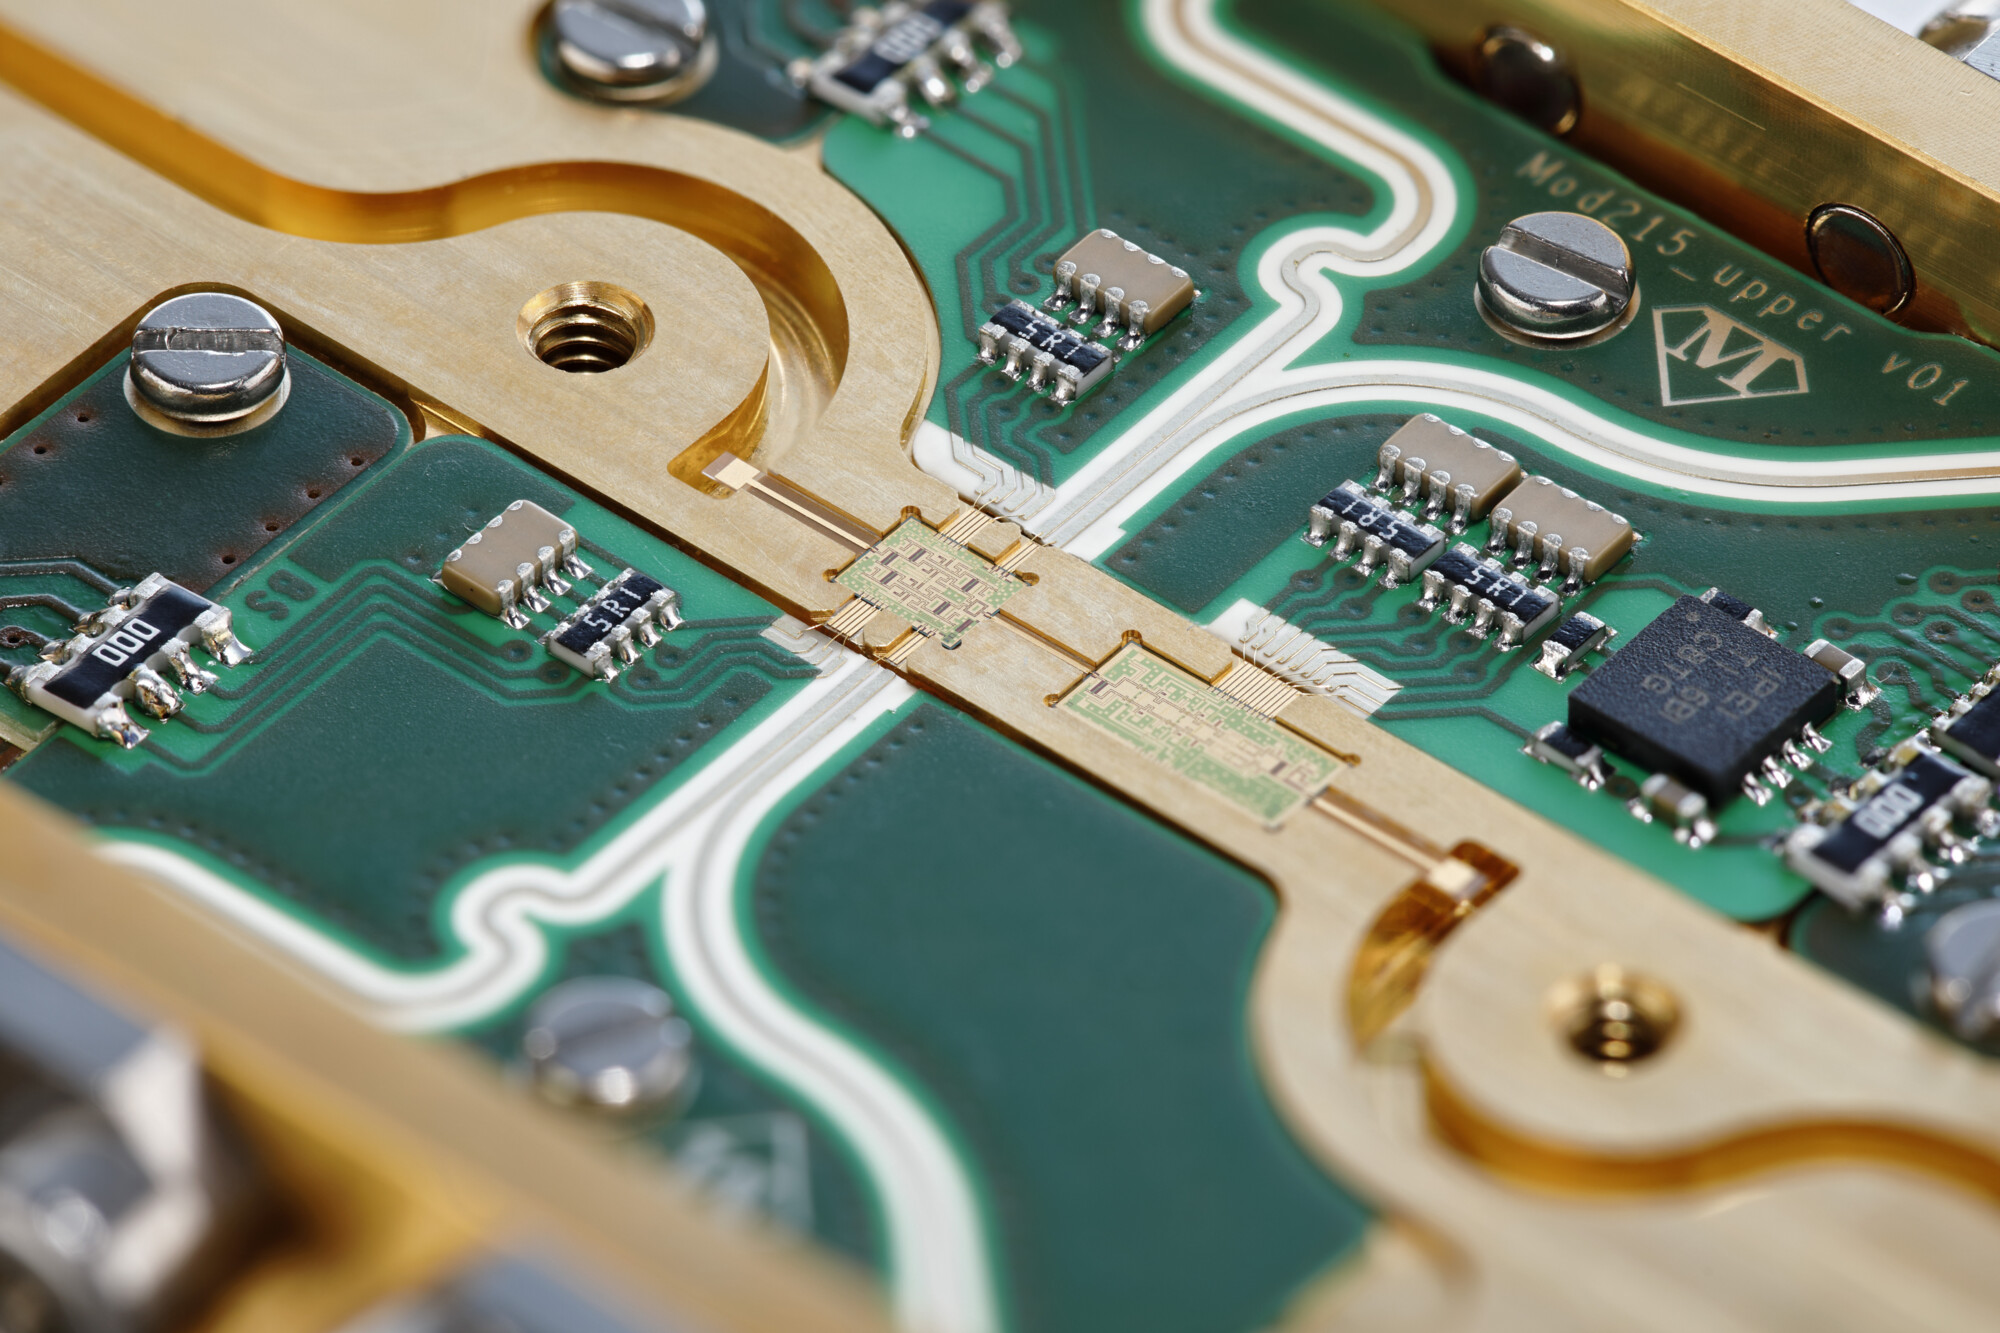
\includegraphics
            [width=\paperwidth, keepaspectratio]
            {pictures/background/background-level-B.jpg}
        };
    \end{tikzpicture}
    }
}

\newcommand\defaultbackground {
    \usebackgroundtemplate{
    \begin{tikzpicture}[remember picture, overlay]
        \node[at=(current page.center)] {
            
\includegraphics
            [width=\paperwidth, keepaspectratio]
            {pictures/background/background-default.pdf}
        };
    \end{tikzpicture}
    }
}

\newcommand\pascalbackground {
    \usebackgroundtemplate{
    \begin{tikzpicture}[remember picture, overlay]
        \node[at=(current page.center)] {
            
\includegraphics
            [width=\paperwidth, keepaspectratio]
            {pictures/background/background-pascal.pdf}
        };
    \end{tikzpicture}
    }
}

\newcommand\maxbackground {
    \usebackgroundtemplate{
    \begin{tikzpicture}[remember picture, overlay]
        \node[at=(current page.center)] {
            
\includegraphics
            [width=\paperwidth, keepaspectratio]
            {pictures/background/background-max.pdf}
        };
    \end{tikzpicture}
    }
}

% -------------- TITLE PAGE --------------
\makeatletter
\setbeamertemplate{title page}
{
    \begin{columns}
        \begin{column}{0.75\textwidth}
            {
                
\includegraphics[scale = 0.35]{pictures/logo/udes_logo.pdf}\\
            }
            \vspace{24pt}
            \begin{tikzpicture}
                \def\boxwidth{\textwidth}
                \def\boxheight{3cm}
                \def\cornerradius{6pt}
                \def\shadowshift{0.5ex}
                
                \node[fill=UDSgreenSolidarite,
                      fill opacity=0.9,
                      rounded corners=6pt,
                      minimum width=1.1\boxwidth, minimum height=\boxheight,
                      text=white,
                      text opacity=1,
                      align=center] (mainbox) at (0, 0){
                    \usebeamerfont{title}
                    \textbf{\inserttitle}\\
                    \usebeamerfont{subtitle}\usebeamercolor[fg]{subtitle}
                    \textbf{\insertsubtitle}\\\\
                    \small\usebeamerfont{author}\insertauthor
                };

                \path (mainbox) node[rectangle, minimum width=1.0999\boxwidth, minimum height=0.996*\boxheight, rounded corners=\cornerradius, save path=\inbox] at (0, 0) {};
                \tikzset{protect=\inbox}

                \begin{scope}[transparency group, opacity=1]
                    \fill[color=black, opacity=0.33, rounded corners=\cornerradius,
                          blur shadow = {shadow xshift=.25ex, shadow yshift=-.25ex}]
                        (-0.5\boxwidth + \shadowshift, 0.5*\boxheight - \shadowshift) rectangle 
                        (0.5\boxwidth + \shadowshift, -0.5*\boxheight - \shadowshift);
                \end{scope}
            \end{tikzpicture}
            \vspace{24pt}
        \end{column}
        \begin{column}{0.25\textwidth}
        \end{column}
    \end{columns}
}
\makeatother


\newcommand\thankyouframe{
    \begin{frame}
    \begin{multicols}{2}
        \begin{beamercolorbox}[sep=8pt, center, shadow=true, rounded=true, wd=0.5\textwidth, bgopacity=0.85]{title}
            \usebeamerfont{title}Merci!\\
        \end{beamercolorbox}%
    \vfill\null
    \columnbreak
    \end{multicols}
\end{frame}
}
